\section{Mehrprozessorsysteme}

\begin{defi}{Flynn'sche Klassifikation}
    Von Flynn wurde 1972 eine sehr grobe aber heute noch häufig genutzte Unterscheidung von Parallelrechnern eingeführt.
    Sie orientiert sich an der Anzahl der gleichzeitig vorhandenen Instruktions- und Datenströme.
    
    Parallelrechner:
    
    \begin{center}
        \begin{tabular}{ll}
            SISD & Single Instruction Single Data (Von Neumann-Rechner $\to$ kein paralleles System) \\
            SIMD & Single Instruction Multiple Data                                                  \\
            MISD & Multiple Instruction Single Data $\to$ \textbf{irrelevant!}                       \\
            MIMD & Multiple Instruction Multiple Data 
        \end{tabular}
    \end{center}
\end{defi}

\begin{bonus}[Flynn'sche Klassifikation]{Erweiterungen}
    \begin{itemize}
        \item \emph{SIMD} Single Instruction Multiple Data
              \begin{itemize}
                  \item Vektor-Prozessoren (auch Mischformen mit MIMD vorhanden!)
                  \item Array-Prozessoren
              \end{itemize}
        \item \emph{MIMD} Multiple Instruction Multiple Data
              \begin{itemize}
                  \item Speichergekoppelte Multiprozessoren
                        \begin{itemize}
                            \item Unified Memory Architecture (UMA)
                            \item Non-Uniform Memory Access (NUMA)
                        \end{itemize}
                  \item Nachrichtengekoppelte Multiprozessoren
                        \begin{itemize}
                            \item Massively Parallel Processing (MPP)
                            \item Cluster Of Workstations (COW)
                        \end{itemize}
              \end{itemize}
    \end{itemize}
\end{bonus}

\subsection{Speichergekoppelte Systeme}

\begin{defi}{Speichergekoppelte Systeme}
    Bei speichergekoppelten Multiprozessoren arbeiten alle Prozessoren in einem einheitlichen Adressraum.
    
    Je nach physiklischer Speicherorganisation unterscheidet man:
    \begin{itemize}
        \item Symmetrische Multiprozessoren (SMP, symmetric multiprocessor),
              bei denen gleichartige Prozessoren über ein Verbindungsnetzwerk mit einem gemeinsamen Speicher verbunden sind
        \item Distributed-Shared-Memory Systeme,
              bei denen zwar ein einheitlicher Adressraum existiert, 
              aber die Speicher physikalisch auf einzelnen Verarbeitungsknoten verteilt sind
    \end{itemize}
    
    \emph{Bemerkungen:}
    \begin{itemize}
        \item Speichergekoppelte Multiprozessoren gelten als einfacher programmierbar gegenüber nachrichtengekoppelten Multiprozessoren
        \item Nutzbare Parallelität reicht von der Programmebene bis zur Blockebene
        \item Autoparallelisierende Compiler nutzen insbesondere die Parallelisierung der Schleifenebene (einzelne Iterationen nebenläufig abarbeitbar)
    \end{itemize}
\end{defi}

\begin{defi}{Uniform Memory Access}
    Kapitel 5 Seite 8
\end{defi}

\begin{defi}{Non-Uniform Memory Access}
    Kapitel 5 Seite 9
\end{defi}

\begin{defi}{Nachrichtengekoppelte Systeme}
    Kapitel 5 Seite 10
\end{defi}

\subsection{Verbindungsnetzwerke}

\begin{defi}{Verbindungsnetzwerk}
    Ein Verbindungsnetzwerk ermöglicht den Datenaustausch (und die Verteilung des Programms) zwischen den Prozessoren.
    
    Um einen hohen Datentransfer zu erhalten, 
    wird eine große Anzahl von Drähten benötigt!
    
    Ein VN gleicht einer Straße:
    \begin{itemize}
        \item Link = Straße
        \item Switch = Kreuzung
        \item Distance/Hops = Anzahl der zurückgelegten Straßenblöcke
        \item Routing algorithm = Reiseplan
    \end{itemize}
    
\end{defi}

\begin{defi}[Verbindungsnetzwerk]{Latenz}
    Zeit für den Transfer zwischen den Knoten
\end{defi}

\begin{defi}[Verbindungsnetzwerk]{Bandbreite}
    \[\frac{\text{transferierte Daten}}{\text{Zeit}}\]
    Bandbeite eines Link: $\text{bw} = w \cdot \frac{1}{t}\frac{\text{bit}}{\text{sec}}$
    mit $w$: Anzahl der Drähte
\end{defi}

\begin{defi}[Verbindungsnetzwerk]{Durchmesser}
    maximale Distanz zwischen zwei beliebigen Prozessoren
\end{defi}

\begin{defi}[Verbindungsnetzwerk]{Topologie}
    Wie sind die Nachbarknoten angeordnet und erreichbar?
\end{defi}

\subsubsection{Statische Verbindungsnetzwerke}

\begin{defi}{Lineare Anordnung}
    \begin{center}
        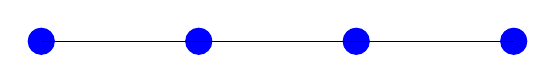
\begin{tikzpicture}
            \node[circle, draw=blue, fill=blue] (d0) at (0, 0) {};
            \node[circle, draw=blue, fill=blue] (d1) at (2, 0) {};
            \node[circle, draw=blue, fill=blue] (d2) at (4, 0) {};
            \node[circle, draw=blue, fill=blue] (d3) at (6, 0) {};
            \draw (d0.center) to[out=0, in=180] (d1.center);
            \draw (d1.center) to[out=0, in=180] (d2.center);
            \draw (d2.center) to[out=0, in=180] (d3.center);
        \end{tikzpicture}
        \\
        Diameter = $N-1$
    \end{center}
\end{defi}

\begin{defi}{Torus oder Ring}
    \begin{center}
        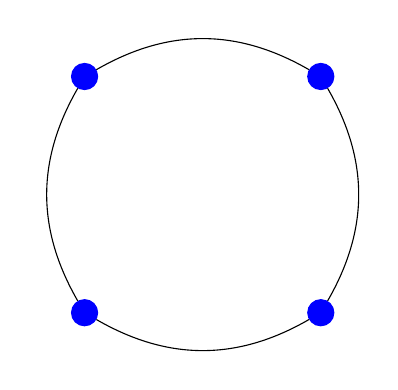
\begin{tikzpicture}
            \node[circle, draw=blue, fill=blue] (d0) at (3.5, 0.5) {};
            \node[circle, draw=blue, fill=blue] (d1) at (3.5, 3.5) {};
            \node[circle, draw=blue, fill=blue] (d2) at (0.5, 3.5) {};
            \node[circle, draw=blue, fill=blue] (d3) at (0.5, 0.5) {};
            \draw (d0) to[bend right] node[left]{}(d1);
            \draw (d1) to[bend right] node[left]{}(d2);
            \draw (d2) to[bend right] node[left]{}(d3);
            \draw (d3) to[bend right] node[left]{}(d0);
        \end{tikzpicture}
        \\
        Diameter = $\frac{N}{2}$
    \end{center}
\end{defi}

\begin{defi}{Torus}
    2D-Torus:
    \begin{center}
        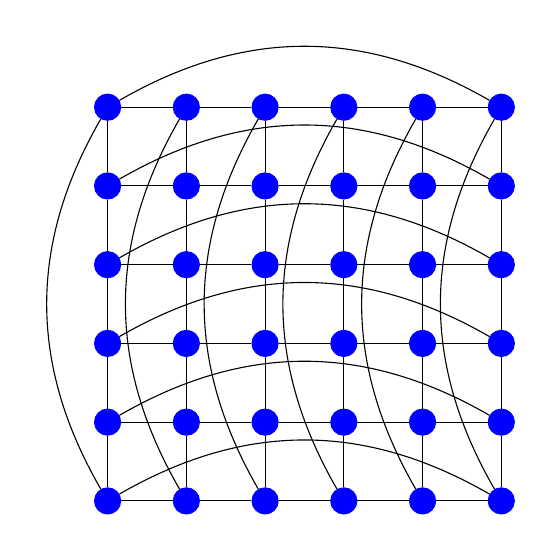
\begin{tikzpicture}[circlestyle/.style={circle, draw=blue, fill=blue}]
            \foreach \x in {0, ..., 5}
            \foreach \y in {0, ..., 5}
            \node[circlestyle] (\x\y) at (\x, \y) {};
            
            \foreach \x in {0,...,5}
            \foreach \y [count=\yi] in {0,...,4}
            \draw (\x\y)--(\x\yi) (\y\x)--(\yi\x); 
            
            \draw (00) to[bend left] node[left]{}(05);
            \draw (10) to[bend left] node[left]{}(15);
            \draw (20) to[bend left] node[left]{}(25);
            \draw (30) to[bend left] node[left]{}(35);
            \draw (40) to[bend left] node[left]{}(45);
            \draw (50) to[bend left] node[left]{}(55);
            
            \draw (00) to[bend left] node[left]{}(50);
            \draw (01) to[bend left] node[left]{}(51);
            \draw (02) to[bend left] node[left]{}(52);
            \draw (03) to[bend left] node[left]{}(53);
            \draw (04) to[bend left] node[left]{}(54);
            \draw (05) to[bend left] node[left]{}(55);
        \end{tikzpicture}
    \end{center}
\end{defi}

\begin{defi}{Gitter}
    2D-Gitter:\\
    Diameter = $2\cdot\left(\sqrt{N} - 1\right)$
    \begin{center}
        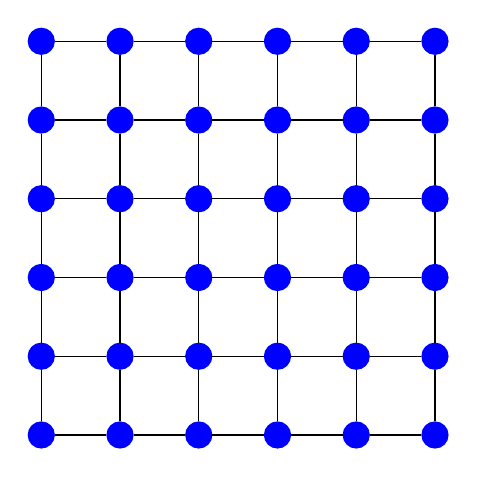
\begin{tikzpicture}[circlestyle/.style={circle, draw=blue, fill=blue}]
            \foreach \x in {0, ..., 5}
            \foreach \y in {0, ..., 5}
            \node[circlestyle] (\x\y) at (\x, \y) {};
            
            \foreach \x in {0,...,5}
            \foreach \y [count=\yi] in {0,...,4}
            \draw (\x\y)--(\x\yi) (\y\x)--(\yi\x); 
        \end{tikzpicture}
    \end{center}
\end{defi}

\begin{defi}{Hypercube}
    \begin{itemize}
        \item Anzahl der Knoten: $N = 2d$
        \item Diameter: $d = \log_2 N$
        \item Greycode Adressierung: Jeder Knoten verbunden mit $d$ anderen Knoten unterscheidet sich durch \emph{ein Bit} in der Adresse
        \item Beispiele: Intel iPSC und NCUBE
        \item 0d:
              
\begin{tikzpicture}[circlestyle/.style={circle, draw=blue, fill=blue}]
                  \node[circlestyle] (A) at (0,0) {};
              \end{tikzpicture}
        \item 1d:
              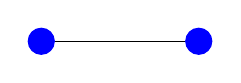
\begin{tikzpicture}[circlestyle/.style={circle, draw=blue, fill=blue}]
                  \node[circlestyle] (A) at (0,0) {};
                  \node[circlestyle] (B) at (2,0) {};
                  \draw (A) to[] node[left]{}(B);
              \end{tikzpicture}
        \item 2d:
              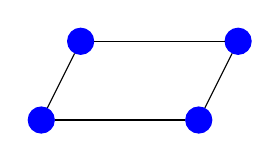
\begin{tikzpicture}[circlestyle/.style={circle, draw=blue, fill=blue}]
                  \node[circlestyle] (A) at (0,0) {};
                  \node[circlestyle] (B) at (2,0) {};
                  \draw (A) to[] node[left]{}(B);
                  
                  \node[circlestyle] (C) at (0.5, 1) {};
                  \node[circlestyle] (D) at (2.5, 1) {};
                  \draw (C) to[] node[left]{}(D);
                  
                  \draw (A) to[] node[left]{}(C);
                  \draw (B) to[] node[left]{}(D);
              \end{tikzpicture}
        \item 4d: TODO!
    \end{itemize}
    TODO: tikzpicture
\end{defi}

\begin{defi}{Baum}
    Diameter = $\log_2 N$
    \begin{itemize}
        \item Planares Layout:
              TODO: tikzpicture
        \item Fetter Baum: (mehr Verbindungen erhöhen das Datenvolumen)
    \end{itemize}
\end{defi}

\begin{bonus}{Übersicht statischer Verbindungsnetzwerke}
    \begin{tabularx}{\textwidth}{|l|X|X|X|}
        \hline
        Topologie          & Anzahl der Verbindungskanäle pro Knoten & Maximale Entfernung (Diameter) & Gesamtanzahl der Verbindungskanäle \\
        \hline
        Ring               & 2                                       & $\frac{N}{2}$                  & $N-1$                              \\
        \hline
        Baum               & 3                                       & $2\cdot (\log_2 N - 1)$        & $N-1$                              \\
        \hline
        2D - Gitter        & 4                                       & $2\cdot \sqrt{N}$              & $2\cdot N$                         \\
        \hline
        3D - Gitter        & 6                                       & $3\cdot \sqrt[3]{N}$           & $3\cdot N$                         \\
        \hline
        Hexagon. Gitter    & 6                                       & $3\cdot \sqrt[3]{N}$           & $3\cdot N$                         \\ 
        \hline
        Hypercube          & $\log_2 N$                              & $\log_2 N$                     & $N \log_2 \frac{N}{2}$             \\
        \hline
        Vollst. Vernetzung & $N - 1$                                 & 1                              & $N \cdot \frac{N-1}{2}$            \\
        \hline
    \end{tabularx}
\end{bonus}

\subsubsection{Dynamische Verbindungsnetzwerke}

\begin{defi}{Bus}
    \begin{itemize}
        \item Durch die wahlweise Zuschaltung einzelner Verarbeitungsknoten zum Datentransfer an einen Bus ist das Bussystem eine typische dynamische Verbindungseinrichtung
        \item Der Bus bildet die Engstelle im busgekoppelten Multiprozessorsystem,
              so dass auch Doppelbusse oder allgemein Mehrfachbusse eingesetzt werden
        \item Bussysteme und auch Mehrbussysteme werden für Systeme mit höchstens 30 Prozessoren eingesetzt,
              um Zugiffskonflikte in Grenzen zu halten
    \end{itemize}
\end{defi}

\begin{defi}{Crossbar}
    \begin{itemize}
        \item $M \times M$ Matrix
        \item einfaches Weiterleiten an mehrere Ausgänge
        \item komplexe Steuerung
        \item Verdrahtungsaufwand
        \item Pufferung bei Blockierungen
        \item Diameter = 1, d. h. beliebige Verbindungen können unter Einsatz jeweils nur einer Schaltzelle realisiert werden
    \end{itemize}
\end{defi}

\begin{defi}{Zellenbasierte Systeme}
    Zellen mit 2 Eingängen und 2 Ausgägen bilden die Basis für solche Systeme.
    \begin{itemize}
        \item 2 Bit $\to$ 4 Schaltzustände
        \item gerade Zellen
        \item kreuzende Zellen
        \item Eingänge mit mehreren Ausgängen verbunden (seltener genutzt)
    \end{itemize}
\end{defi}

\begin{defi}{Einstufige Netzwerke}
    Eine Spalte von Schaltzellen wird durch Rückkopplung der Ausgänge auf die Eingänge Verbunden. 
    Die Zellen werden mehrfach durchlaufen.
\end{defi}

\begin{defi}{Mehrstufige Netzwerke}
    Mehrere Spalten von Schaltzellen, auch mit Rückführungen, 
    sind fest miteinander verbunden.
\end{defi}

\begin{defi}{Omega-Netzwerk}
    TODO: Including images does not work!
    % \begin{figure}[H]
    %     \centering
    %     \includegraphics{graphics/OmegaNetwork.jpg}
    %     \caption{By Bjmyers17, CC BY-SA 3.0, https://commons.wikimedia.org/w/index.php?curid=75639225}
    % \end{figure}
\end{defi}

\begin{defi}{Benes-Netzwerk}
    TODO: Including images does not work!
    % \begin{figure}[H]
    %     \centering
    %     \includegraphics{graphics/Benesnetwork.png}
    %     \caption{By Piggly - Own work, Public Domain, https://commons.wikimedia.org/w/index.php?curid=2988080}
    % \end{figure}
\end{defi}

\subsubsection{Cluster-Interconnects}

\begin{defi}{Cluster-Interconnect}
    
\end{defi}

\begin{defi}{Infiniband}
    \begin{itemize}
        \item \ldots ist eine Architektur für Hochgeschwindigkeitsverbindungen zwischen Rechnern und externen Speicherservern.
        \item \ldots wurde unter Führung von Intel entwickelt, später Mellanox, jetzt Nvidia.
        \item \ldots eignet sich auch als Verbindungsnetzwerk von Rechen-Clustern.
    \end{itemize}
    aktuell: Infiniband EDR / HDR mit bis zu 200 Gbit/s
\end{defi}

\begin{defi}{Gigabit Ethernet}
    \begin{itemize}
        \item \ldots wird vorwiegend in lokalen Netzwerken genutzt,
              auch für Heimanwender mit RJ45 Stecker für Kupferkabel (z.B. Lan-Buchsen am Router)
        \item \ldots ist für Glasfaser und (twisted-pair) Kupferkabel spezifiziert,
              höhrere Bandbreiten aber nur über Glasfaser umsetzbar: bis zu 100 Gb/s
        \item \ldots ist Switch-basiert und abwärtskompatibel
        \item \ldots nutzt spezielle Kollisionserkennung / -vermeidung,
              wie CSMA / CD (Carrier Sense Multiple Access with Collision Detection)
    \end{itemize}
\end{defi}

\begin{defi}[Verbindungsnetzwerk]{Klassifikation}
    \begin{itemize}
        \item Statisch
              \begin{itemize}
                  \item Ein-dimensional
                  \item Zwei-dimensional
                  \item Mehr-dimensional
              \end{itemize}
        \item Dynamisch
              \begin{itemize}
                  \item Bussysteme
                  \item Zellenbasierte Netze
                        \begin{itemize}
                            \item Einstufig
                            \item Mehrstufig
                                  \begin{itemize}
                                      \item Blockierend
                                      \item Nicht-Blockierend
                                  \end{itemize}
                        \end{itemize}
                  \item Kreuzschienenverteiler (Crossbars)
              \end{itemize}
    \end{itemize}
\end{defi}

